% !TEX root = ../om_ts_002.tex

\begin{frame} % название фрагмента

\videotitle{MA Process}

\end{frame}



\begin{frame}{MA Process: Plan}
	\begin{itemize}[<+->]
		\item Definition and notations with lags
		\item Stationarity
		\item Predictability
		\item Reversibility
	\end{itemize}
	
\end{frame}

\begin{frame}
	\frametitle{Lag operator}
	
	\begin{block}{Definition}
		For the process $(y_t)$ defined at $t \in \mathbb{Z}$, \alert{lagged} process
		$L y_t$ is the same sequence of values ​​with a shifted index,
		\[
		L y_t = y_{t-1}
		\]
	\end{block}
	
	\pause
	\[
	L^2 y_t = L\cdot L\cdot y_t = L\cdot y_{t-1} = y_{t-2}
	\]
	\pause
	\[
	\Delta y_t = y_t - y_{t-1} = (1 - L) y_t
	\]
	\pause
	\[
	\Delta_{12} y_t = y_t - y_{t-12} = (1 - L^{12}) y_t
	\]
\end{frame}

\begin{frame}
	\frametitle{MA process}
	
	\begin{block}{Definition}
		Process $(y_t)$, which \alert{can} be represented as
		\[
		y_t = \mu + u_t + \alpha_1 u_{t-1} + \ldots + \alpha_q u_{t-q},
		\]
		where $\alpha_q \neq 0$ and $(u_t)$ is white noise, is called the $MA(q)$ process
	\end{block}

	\alert{MA — Moving Average}
	
	
	\pause
	Example $MA(1)$ process:
	\[
	y_t = 5 + u_t + 0.3 u_{t-1},
	\]
	where $(u_t)$ is some white noise

	
\end{frame}


\begin{frame}
	\frametitle{Notation with lags}
	
	\begin{block}{MA with lag polynomial}
		Process $(y_t)$, which \alert{can} be represented as
		\[
		y_t = \mu + P(L) u_t,
		\]
		where $P(L)$ is a polynomial of degree $q$ in lag $L$ with $P(0)=1$, and $(u_t)$ is white noise,
		is called $MA(q)$ a process
	\end{block}
	
	\pause
	An example $MA(2)$ process:
	\[
	y_t = 5 + (1 - 0.2 L + 0.3 L^2) u_t,
	\]
	where $(u_t)$ is white noise
\end{frame}





\begin{frame}
	\frametitle{ACF and Forecasts}
	
	Traditionally $MA(q)$ process is evaluated assuming joint normality of $(y_t)$.
	
	\pause
	Zero $\rho_k=0$ for $k>q$ implies independence of $y_t$ and $y_{t+k}$.
	
	\pause
	Forecasts more than $q$ steps ahead are exactly the same.
	
	\[
	(y_{T+q + 1} \mid \mathcal{F}_T) \sim (y_{T+q + 2} \mid \mathcal{F}_T) \sim (y_{T+q + 3} \mid \mathcal{F}_T) \sim \ldots
	\]
\end{frame}

\begin{frame}
	\frametitle{Predictions for $MA(2)$}
	
	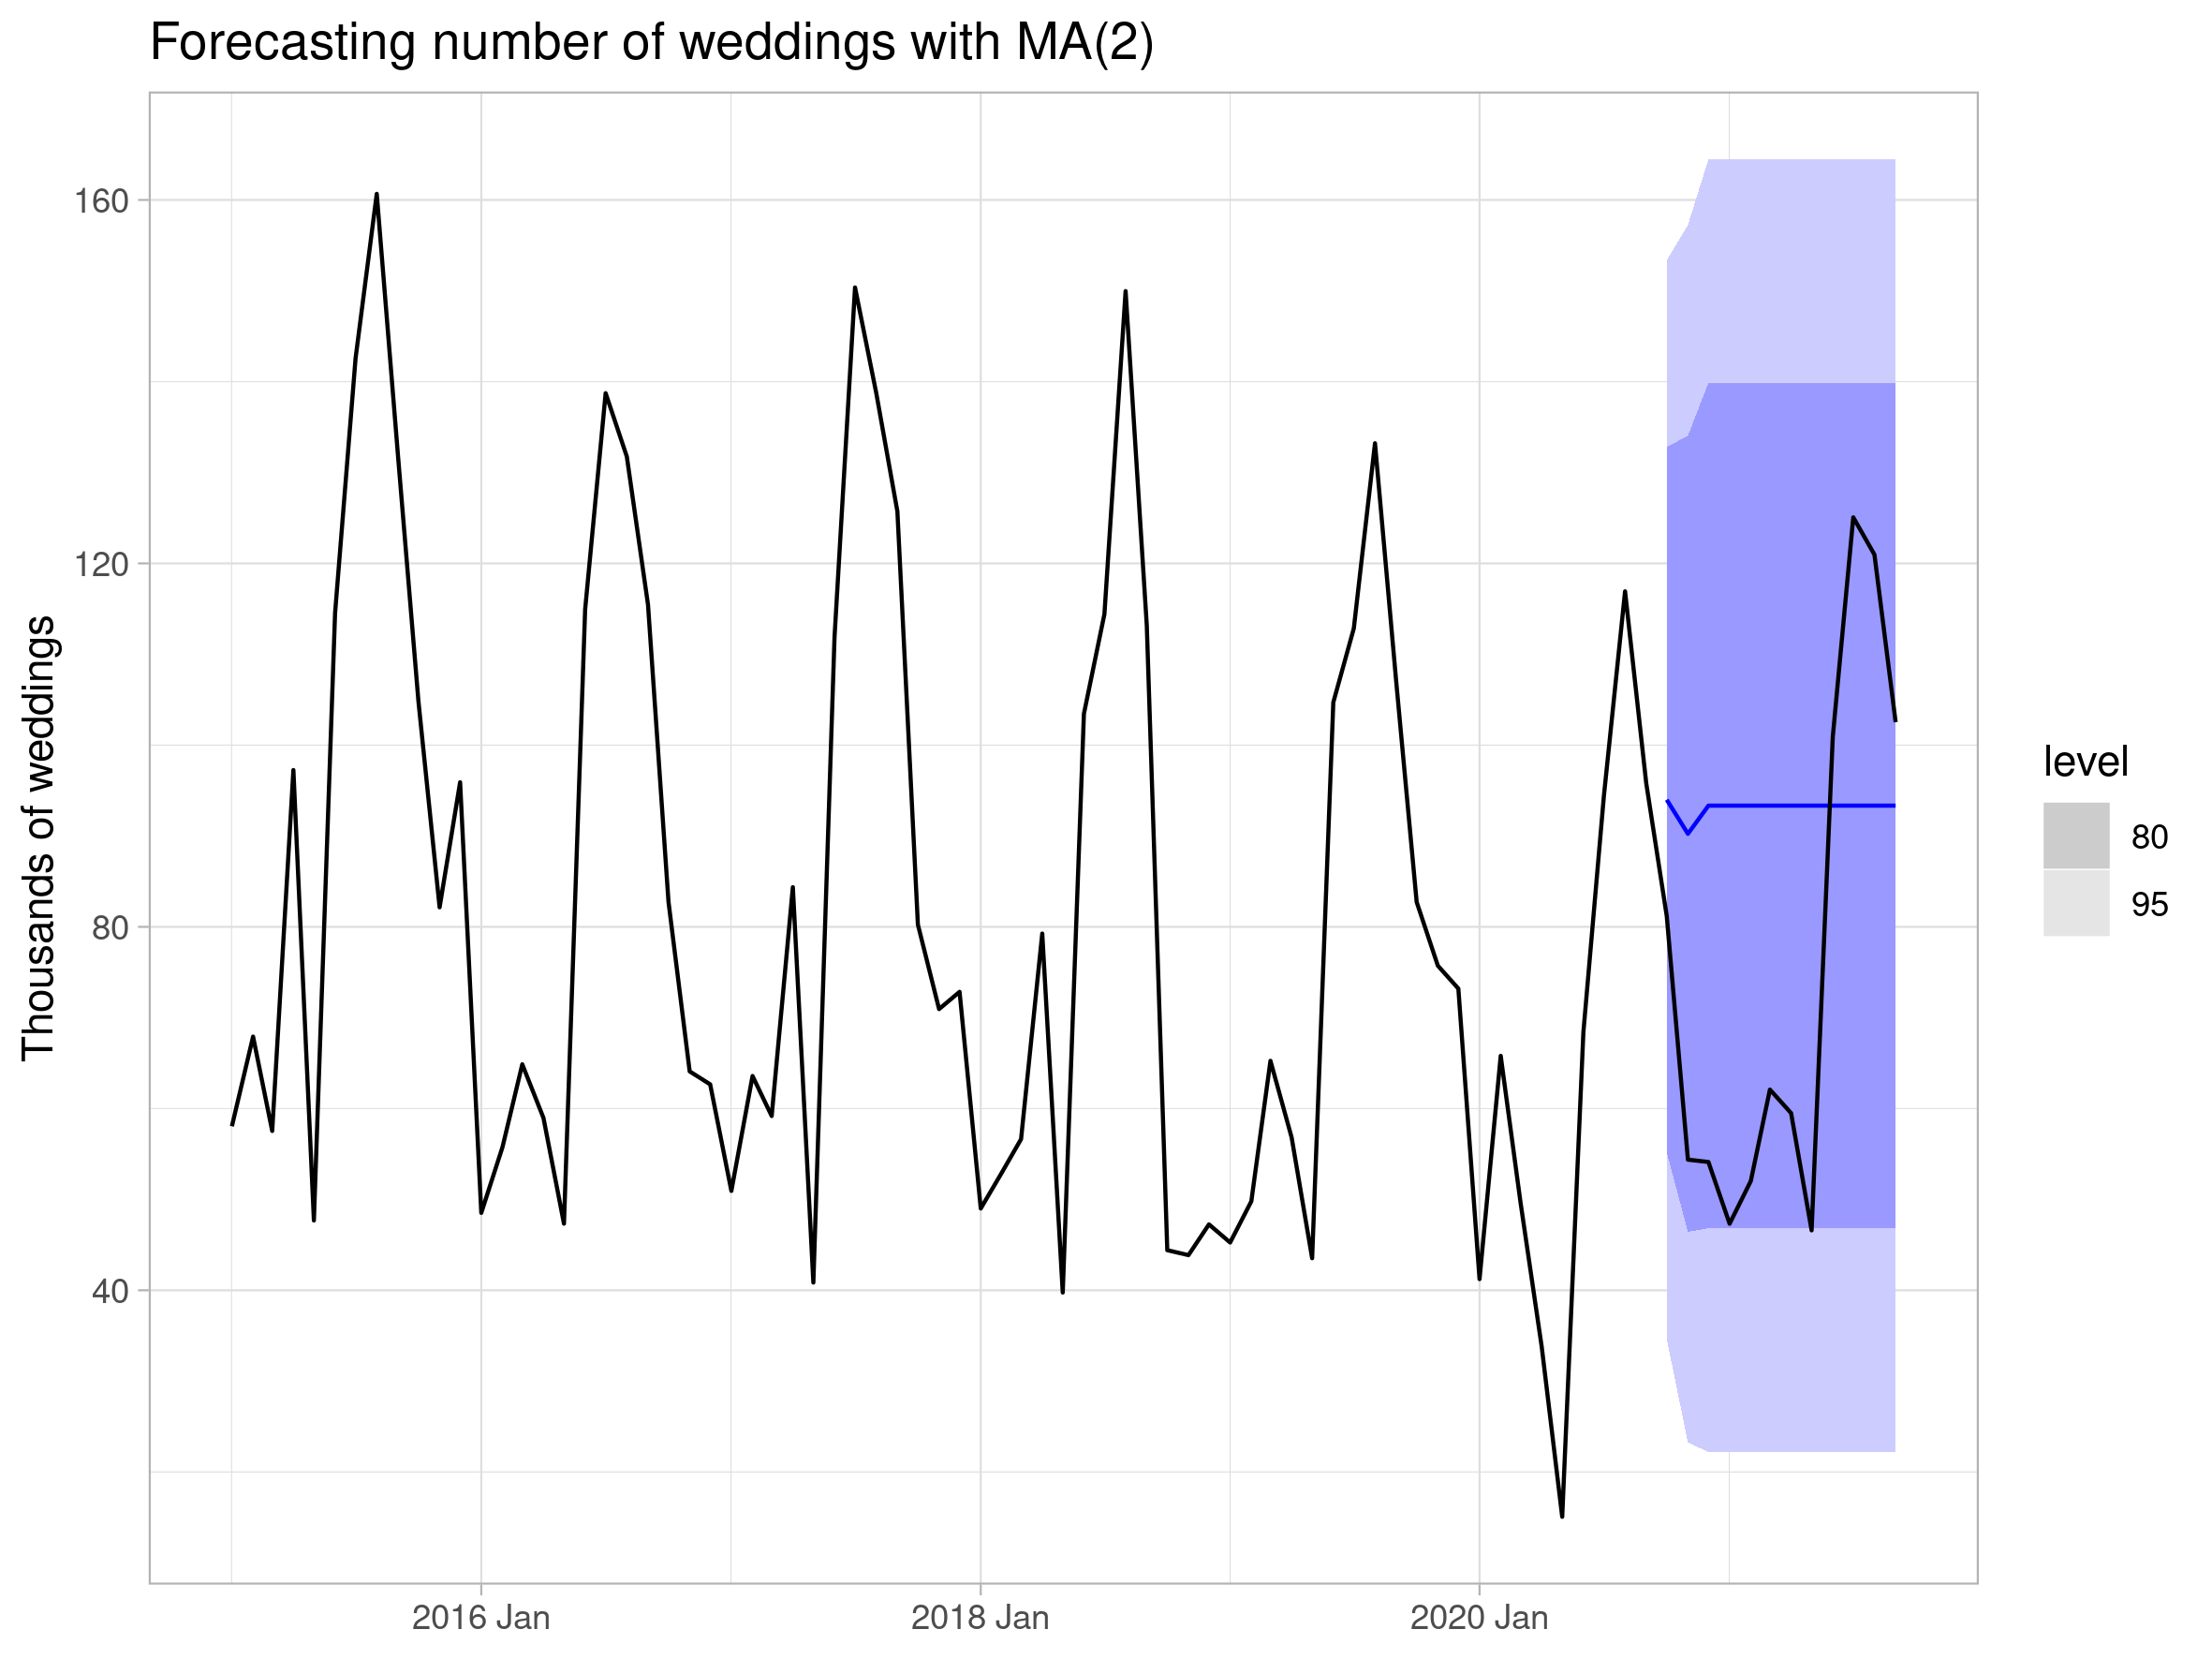
\includegraphics[width=\textwidth]{pictures/om_ts_04-094.png}
	
	
\end{frame}




\begin{frame}
	\frametitle{$MA(\infty)$}
	
	\begin{block}{Definition}
		Process $(y_t)$, which \alert{can} be represented as
		\[
		y_t = \mu + u_t + \alpha_1 u_{t-1} + \alpha_2 u_{t-2} + \ldots,
		\]
		where $(u_t)$ is white noise, an infinite number of $\alpha_i \neq 0$ and
		$\sum_{i=1}^{\infty} \alpha_i^2 < \infty$,
		is called the $MA(\infty)$ process
	\end{block}
	
	\pause
	$MA(\infty)$:
	\[
	y_t = 5 + u_t + 0.5 u_{t-1} + 0.5^2 u_{t-2} + 0.5^3 u_{t-3} + \ldots
	\]
	
	\pause
	And \alert{this is not allowed}:
	\[
	y_t = 5 + u_t + \frac{1}{\sqrt{2}}u_{t-1} + \frac{1}{\sqrt{3}} u_{t-2} + \frac{1}{ \sqrt{4}} u_{t-3} + \ldots
	\]
	
\end{frame}

\begin{frame}
	\frametitle{Convergences}
	\begin{block}{Theorem}
		If a
		$\sum_{i=0}^{\infty} \alpha_i^2 < \infty$ and $(u_t)$ is a zero-mean stationary process,
		then the sequence of partial sums $y^q_t$ of the form
		\[
		y^q_t = \mu + \sum_{i=0}^q \alpha_i u_{t-i}
		\]
		converges for $q \to \infty$ \alert{in mean}, \alert{in probability}, and \alert{in distribution}
	\end{block}
	
	Nuance: the convergence of the weighted sum is guaranteed for the stationary $(u_t)$
	\pause
	\begin{block}{Bonus}
		\ldots and the resulting process $(y_t)$ is stationary
	\end{block}
\end{frame}



\begin{frame}
	\frametitle{Wald's Theorem}
	
	\begin{block}{Theorem}
		If $(y_t)$ is a stationary process, then it can be represented as:
		\[
		y_t = \sum_{i=0}^{\infty} \alpha_i u_{t-i} + r_t,
		\]
		where
		\begin{itemize}
			\item $(u_t)$ — white noise,
			\item $\sum \alpha_i^2 < \infty$,
			\item $r_t$ is a linear \alert{predictable} random process,
			\item $\Cov(u_t, r_t) = 0$
		\end{itemize}
	\end{block}
	
	
\end{frame}

\begin{frame}
	\frametitle{Predictable Process}
	
	
	\begin{block}{Correct definition}
		A process $(r_t)$ is called \alert{linearly predictable} if
		\begin{itemize}
			\item $(r_t)$ is stationary,
			\item $r_t = \beta_0 + \beta_1 r_{t-1} + \beta_2 r_{t-2} + \ldots + \beta_p r_{t-p}$
		\end{itemize}
		
	\end{block}
	
\end{frame}




%\begin{frame}{$MA(\infty)$: summary}
%	
%	\begin{itemize}[<+->]
	%		\item \alert{Fast} coefficients tending to zero.
	%		\item \alert{Stationary process}.
	%		\item \alert{It's not clear yet how to evaluate.
		%		\end{itemize}
	%\end{frame}







\begin{frame}
	\frametitle{Reversibility condition}
	
	\begin{block}{Characteristic representation}
		The equation $MA(q)$ of the process satisfies the reversibility condition if
		the characteristic polynomial $\phi(\lambda)$ has all roots $\abs{\lambda_i} <1$
	\end{block}
	
	\pause
	
	\begin{block}{Lag representation}
		The equation $MA(q)$ of the process satisfies the reversibility condition if all roots  of 
		the lag polynomial $P(L)$ are  $\abs{\ell_i} >1$
	\end{block}
	
	
\end{frame}

\begin{frame}
	\frametitle{Example of reversible notation $MA(1)$}
	
	\[
	y_t = 5 + u_t + 0.5 u_{t-1}, \quad \sigma^2_u = 4
	\]
	\pause
	\[
	\lambda^1 + 0.5 \cdot \lambda^0
	\]
	\[
	\phi(\lambda) = \lambda + 0.5
	\]
	\pause
	\[
	\lambda_1 = -0.5
	\]
	
\end{frame}


\begin{frame}
	\frametitle{Example of $MA(1)$ irreversible notation}
	
	\[
	y_t = 5 + u_t + 2 u_{t-1}, \quad \sigma^2_u = 1
	\]
	\pause
	\[
	\lambda^1 + 2 \cdot \lambda^0
	\]
	\[
	\phi(\lambda) = \lambda + 2
	\]
	\pause
	\[
	\lambda_1 = -2
	\]
\end{frame}


\begin{frame}
	\frametitle{Nuance}
	
	\begin{block}{Difference}
		Stationarity is a property of the $(y_t)$ process itself.
		
		Reversibility is a property of the equation (process  notation) for~$(y_t)$.
	\end{block}
	
	\pause
    $MA(q)$ has a single notation when reversible
	
\end{frame}



\begin{frame}
\frametitle{MA process: Summary}
	
	\begin{itemize}[<+->]
		\item $MA(q)$ — weighting of several white noises
		\item $MA(q)$ is a stationary process
		\item $ACF$ vanishes sharply, $PACF$ tends to zero
 		\item Reversibility condition: roots of the characteristic polynomial $\abs{\lambda_i} < 1$ or 
		roots of the lag polynomial $\abs{\ell_i} > 1$.
	\end{itemize}
\end{frame}
